\chapter{Elementi di memoria}
	Di fondamentale importanza per l'utilizzo pratico è realizzare dei circuiti con funzionalità di memoria che permettano di immagazzinare accessibili al calcolatore per l'elaborazione. Nel capitolo precedente sono state mostrate dei tipi di circuiti in grado di memorizzare dati binari (come i latch e i flip-flop), tuttavia essi hanno utilità pratica nell'implementazione di circuiti combinatori con funzioni specifiche, ma non sono adatti a realizzare circuiti di memoria in quanto richiedono un numero elevato di transistor e dunque di ingombro su chip (rispetto alle soluzioni che verranno qua esposte).
	
	In primo luogo verranno descritti i principali componenti per la gestione dei conflitti di tensione nell'interconnessione di diversi componenti digitali, ossia i \textit{tri-state buffer}. Verranno poi analizzate due principali celle di memoria \textit{RAM} (\textit{Random Access Memory}), ossia la versione statica più performante e la versione dinamica più piccola.
	
\section{Tri-state buffer}
	
	I sistemi digitali sono realizzati mediante un'interconnessione di diverse sezioni circuitali (come i vari sommatori e moltiplicatori binari, ma anche registri) che tuttavia devono avere la possibilità di comunicare opportunamente. Tutti questi elementi sfruttano il cosiddetto \textit{bus dati} per condividere le informazioni, tuttavia è necessario implementare un sistema che sia in grado di stabilire quale circuito sia in grado di scrivere e/o leggere le informazioni sul bus dati. Questa operazione è necessaria per evitare il problema del \textit{bus contention} dovuta ad una scrittura simultanea di circuiti. Se infatti due sezioni circuitali provassero a imporre una tensione logica diversa, allora sul bus dovrebbe scorrere un'elevata quantità di corrente in quanto la resistenza del circuito è pressoché nulla rispetto alla differenza di tensione cui il bus è sottoposto.
	
	Tale funzione viene realizzata tramite i cosiddetti \textit{tri-state buffer} (e \textit{inverter}), ossia buffer a tre possibili stati che, tramite un apposito segnale di abilitazione in ingresso, permettono (o meno) il passaggio del segnale in ingresso al bus dati. La tabella di verità realizzata può essere schematizzata come
	\begin{center}
	\begin{tabular}{cc|c|c}
		$In$ & $En$ & $Out$ buffer & $Out$ inverter \\ \hline
		0 & 1 & 0 & 1 \\
		1 & 1 & 1 & 0 \\
		0 & 0 & Hi-Z & Hi-Z \\
		1 & 0 & Hi-Z & Hi-Z \\
	\end{tabular}			
	\end{center}

	Come si osserva nel caso di segnale di abilitazione alto, il buffer permette di avere un'uscita che corrisponde al valore logico in ingresso (l'invertitore avrà invece l'uscita negata). La peculiarità interessante del circuito è invece è quanto il segnale di abilitazione è basso: in questo caso l'uscita (rispetto all'ingresso) si pone in una condizione di alta impedenza, "scollegando" l'ingresso dall'uscita e rendendo le due non influenzabili.
	
	La tabella di verità mostra un componente tri-state che permette la comunicazione se il segnale di abilitazione è alto, tuttavia è anche possibile realizzare dei circuiti che richiedono un segnale di abilitazione basso per il trasferimento dell'ingresso.
	\vspace{5mm}
	
	L'implementazione circuitale di un invertitore tri-state è piuttosto semplice ed è rappresentata in figura \ref{fig:tsi:sch} ed è composto sostanzialmente da una serie di 2 p-mos e 2 n-mos opportunamente pilotati.
	
	\begin{figure}[bht]
		\centering
		\begin{subfigure}{0.48\linewidth}
			\centering
			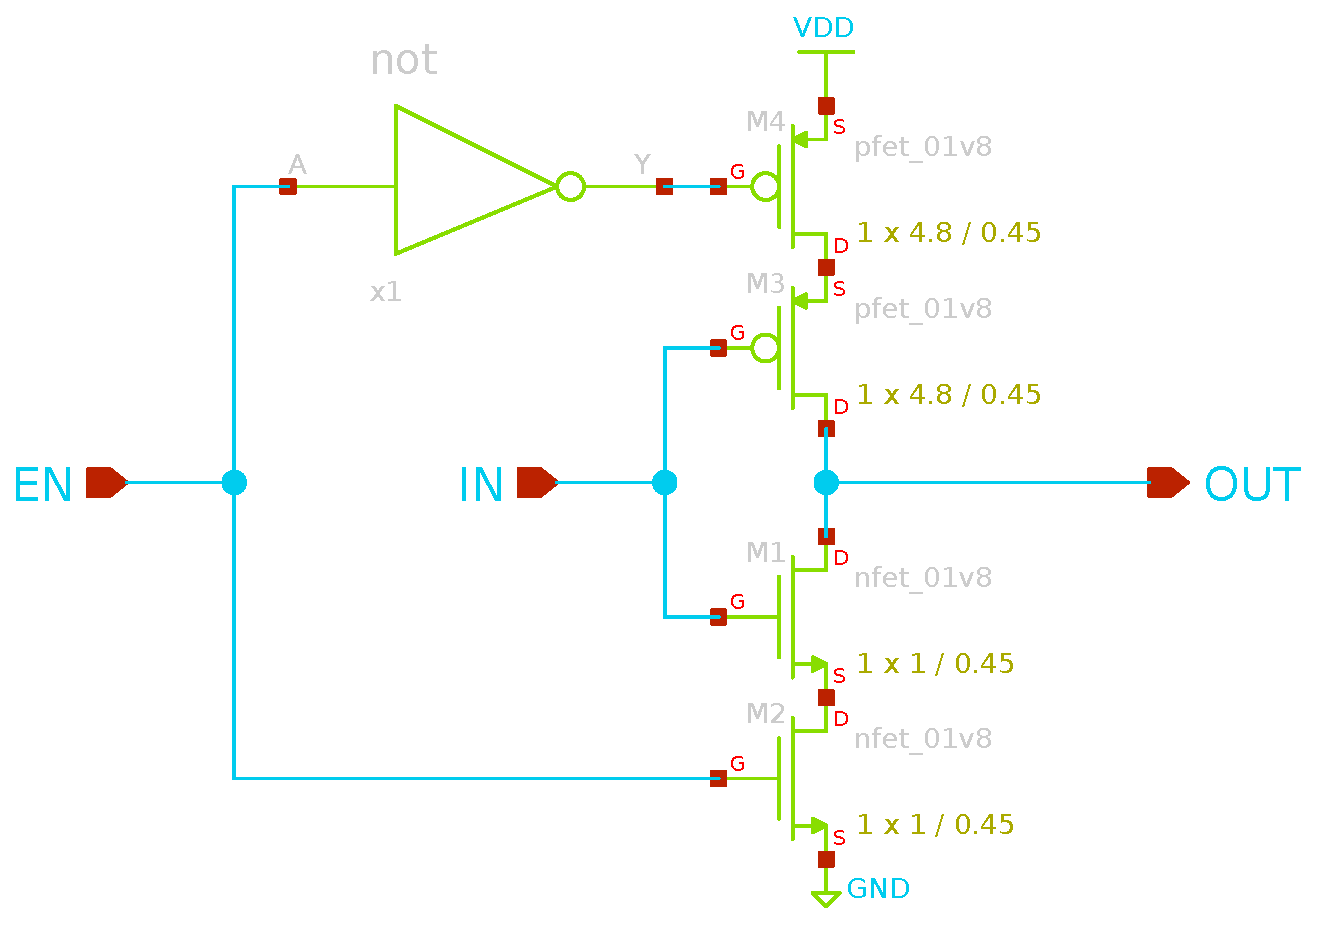
\includegraphics[width=7cm]{Immagini/tri-state-sch}
			\caption{}
		\end{subfigure}
		\begin{subfigure}{0.48\linewidth}
			\centering
			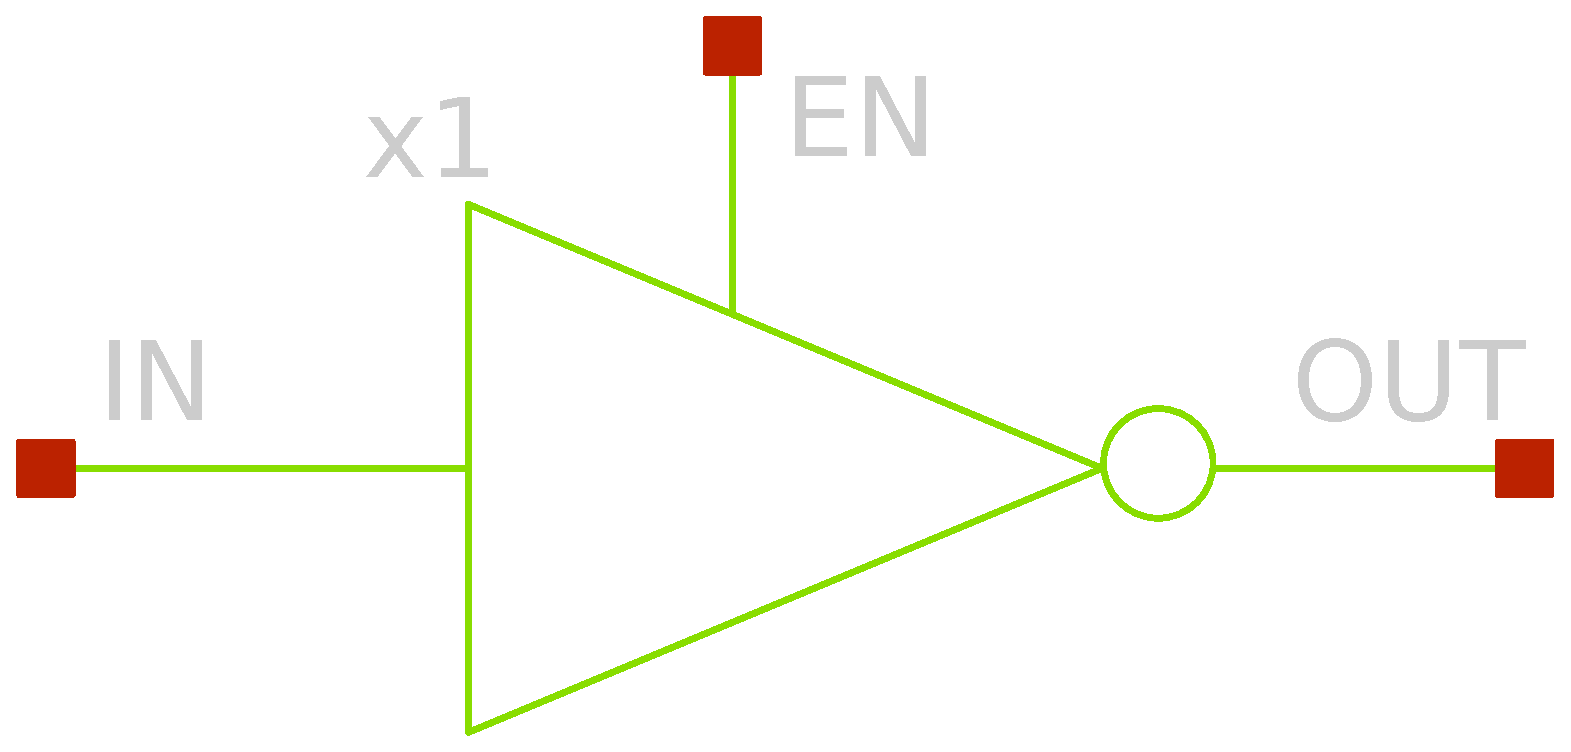
\includegraphics[width=3cm]{Immagini/tri-state-simple}
			\caption{}
		\end{subfigure}
		\caption{schematico (a) e relativa rappresentazione (b) di un invertitore tri-state.}
		\label{fig:tsi:sch}
	\end{figure}

	In particolare si osserva che i due transistor più interni, collegati all'ingresso dei dati, determinano di fatto un invertitore c-mos. L'aspetto che caratterizza il circuito invece è dato dai transitor più esterni collegati all'ingresso di abilitazione $EN$ (segnale che per il p-mos viene negato). Il funzionamento del circuito può dunque essere analizzato per casi:
	\begin{itemize}
		\item nel caso in cui l'ingresso di abilitazione si trovi allo stato logico alto, allora i transistori ad essi associati risultano entrambi contemporaneamente "accessi", permettendo lo scorrimento di corrente. L'uscita è dunque determinata dall'invertitore compreso tra le uscite;
		
		\item nel caso in cui l'ingresso di abilitazione si trovi allo stato logico basso invece i transistor associati risultano interdetti: questo di fatto pone in interdizione il circuito dell'invertitore che indipendentemente dall'ingresso non può permettere uno scorrimento di corrente e dunque l'uscita è posta in alta impedenza rispetto all'ingresso.
	\end{itemize}
	
	Un tri-state buffer viene realizzato a partire dal tri-state inverter ponendo in serie all'uscita un invertitore logico.
	
	
\section{RAM statica}
	Le memorie \textit{RAM}, \textit{Random Access Memory}, mantengono il loro nome per motivi storici e sono caratterizzate dall'avere tempo di accesso ai dati costante indipendentemente dalla posizione degli stessi nello slot di memoria (al contrario di altri tipi di memorie). Questo tipo di memorie sono definite volatili in quanto non adatte a conservare dati, i quali verranno persi non appena verrà tolta l'alimentazione al circuito.
	
	Allo stato attuale le memorie ram possono essere catalogate come \textit{dinamiche}, ossia che richiedono un continuo aggiornamento dei dati immagazzinati per mantenere attive le informazioni salvate, e che costituiscono i moduli di memoria ram commerciali per i computer attuali. Esiste anche la memoria di tipo \textit{statico} che al contrario del caso precedente non richiede un aggiornamento del modulo per mantenere le informazioni ed è dunque più veloce (al costo di un costo come numero di transistor e ingombro su chip maggiore) e per questo è utilizzata all'interno dei microprocessori per realizzare le memorie cache di livello 1, 2 e 3.
	
	\vspace{5mm}
	
	Una cella da 1 bit di memoria statica, abbreviata generalmente come \textit{s-ram}, è costituita da un anello di invertitori logici (che permettono di immagazzinare le informazioni digitali) e da due n-mos in grado di controllare quando la cella è in grado di leggere/scrivere le informazioni sul bus dati e la realizzazione schematica è riportata in figura \ref{fig:sram:sch}.
	
	\begin{figure}[bht]
		\centering
		\begin{subfigure}{0.48\linewidth}
			\centering
			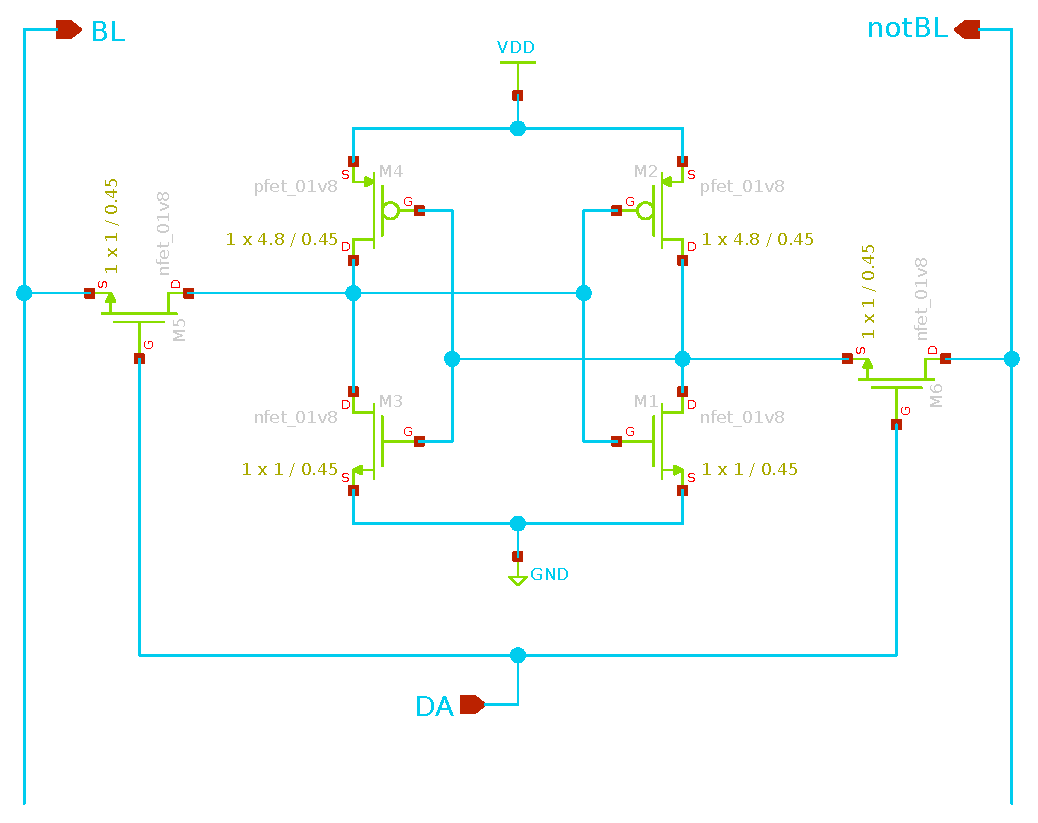
\includegraphics[width=7cm]{Immagini/sram-1bit}
			\caption{}
		\end{subfigure}
		\begin{subfigure}{0.48\linewidth}
			\centering
			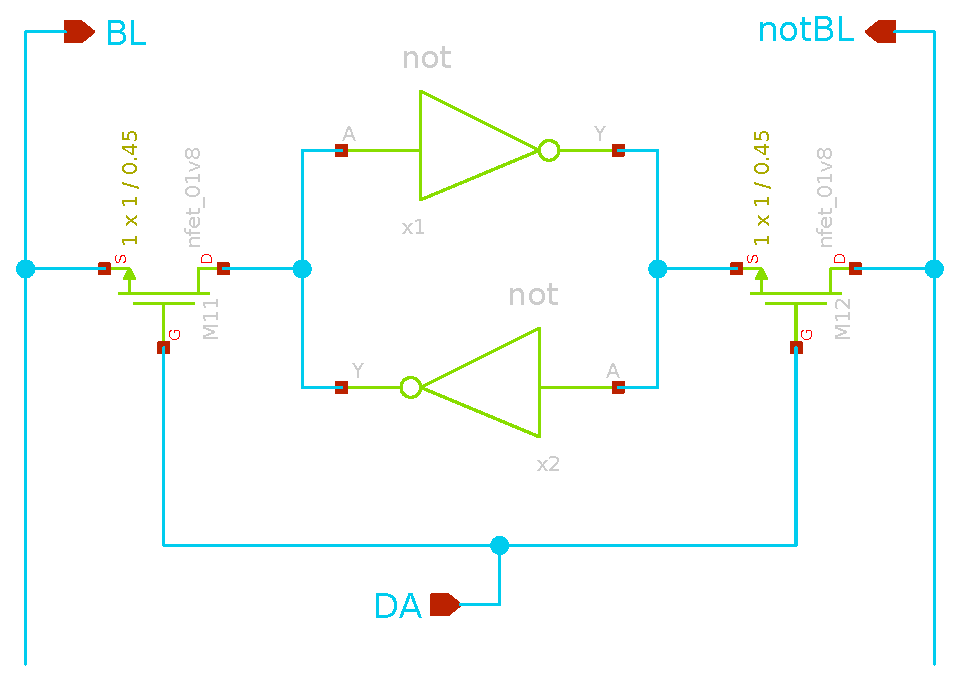
\includegraphics[width=5cm]{Immagini/sram-1bit-simple}
			\caption{}
		\end{subfigure}
		\caption{implementazione circuitale di una cella ad un bit di una ram statica (a). Nella figura (b) è evidenziato l'anello di invertitori logici.}
		\label{fig:sram:sch}
	\end{figure}

	Rispetto allo schematico è possibile osservare come la cella di memoria sia collegata a due cosidette \textit{bit lines} $BL$ il cui ruolo logico si dimostra essere complementare. Nel momento in cui il segnale di \textit{data access} $DA$ viene posto al valore logico alto allora i due n-mos che determinano la connessione dell'anello di invertitori con il bus dati permettono di eguagliare le tensioni delle due parti.
	
	La funzione di memoria viene realizzata dall'anello di invertitori logici: la loro concatenazione in anello chiuso rafforza la differenza di stato logico dei due componenti. Considerando infatti che la parte a sinistra del circuito si trovi ad uno stato logico alto (rispetto alla figura \ref{fig:sram:sch}.b), percorrendo l'anello in senso orario si osserva che l'invertitore impone un segnale logico basso alla parte a destra, che a sua volta rafforzerà il segnale logico alto della parte a sinistra.
	
	Si spiega così la dualità delle due bit lines: l'anello di invertitori determina espressamente due uscite che sono necessariamente allo stato logico complementare.
	
	Pilotando le bit lines è dunque possibile, abilitando la comunicazione della cella dati, scrivere le informazioni dal bus dati nella memoria statica; al contrario se la linea dati non è pilotata sarà la cella a pilotare le bit lines.
	
	\vspace{5mm}
	Le memorie attuali sono ottenute collegando alle stesse bit lines un'elevata quantità di celle elementari il cui accesso (che può essere effettuato solo per una cella ad ogni istante) può essere determinata da una logica di decodifica come un multiplexer. Una struttura così implementata permette di immagazzinare solamente dati ad 1 bit, tuttavia è sufficiente porre in parallelo un numero congruo di queste strutture per realizzare sistemi di memoria per un numero maggiore di bit.
	
\section{RAM dinamica}	
	La memoria ram dinamica (abbreviata d-ram), come già affermato, presenta un tempo di accesso ai dati inferiore rispetto alla controparte statica in quanto è necessario aggiornare ad una determinata frequenza tutte le celle di memoria.
	
	La cella elementare della ram dinamica è caratterizzata dalla presenza di un solo transistor e di una capacità che funge di fatto come dispositivo di memorizzazione delle informazioni.
	
	\begin{figure}[bht]
		\centering
		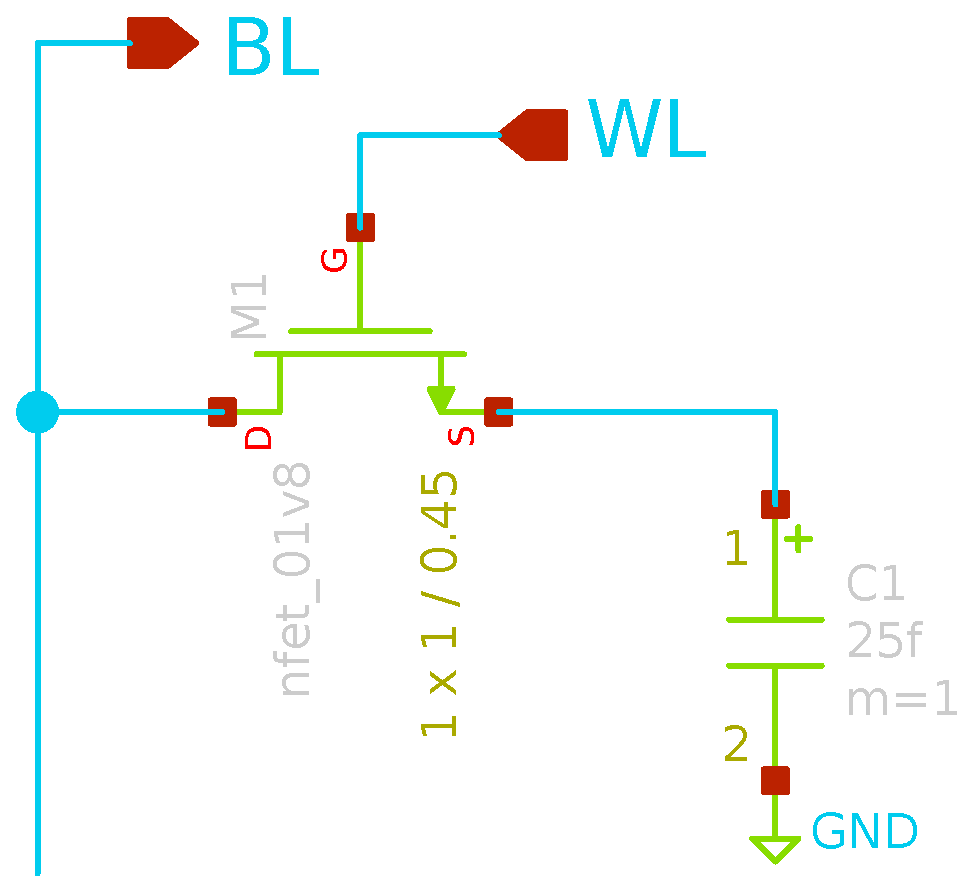
\includegraphics[width=3cm]{Immagini/dram-sch}
		\caption{implementazione circuitale di una cella di memoria d-ram ad un bit.}
		\label{fig:dram:sch}
	\end{figure}

	Il funzionamento del circuito può essere analizzato in riferimento allo schema di una cella di memoria dinamica mostrato in figura \ref{fig:dram:sch}. Come nel caso della controparte statica, le operazioni di lettura/scrittura dati avvengono su una bit line $BL$ e l'abilitazione alla comunicazione (mediante il segnale word line $WL$) avviene tramite un n-mos. Il bit di informazione è associato, come detto, alla carica di un condensatore (che rispetto alle celle di memoria degli anni Novanta, il valore nominale è di circa $25-30fF$ \cite{raminfo}). La bit line può infatti effettuare un'operazione di scrittura sul transistor imponendo la tensione differenziale ai suoi capi che potrà poi essere successivamente letta dalla linea stessa (se essa non viene pilotata da altri circuiti).
	
	Il problema di questo tipo di circuito è che la capacità non è un dispositivo reale e dunque nel tempo è destinata a scaricarsi per via delle correnti parassite. La memoria è detta dinamica per la necessità di eseguire delle operazioni di \textit{refresh}, ossia di ri-aggiornamento dei dati di tutte le celle per evitare di perdere informazioni. Ogni scheda di memoria d-ram è infatti sottoposta a cicli periodici di lettura di tutte le celle con conseguente riscrittura dello stato logico connesso. Questo introduce necessariamente delle latenze nella comunicazione e trasmissione dei dati.
	
	La valutazione delle prestazioni delle memorie ram era inizialmente calcolata in base al tempo di accesso ai dati (in funzione dell'operazione che si vuole eseguire) con valori che potevano variare dai $20-30ns$ a $80-90ns$ \cite{raminfo}. Le memorie dinamiche attualmente utilizzate sui pc, appartenenti allo standard DDR \textit{Double Data Rate}, sono invece caratterizzate principalmente dalla frequenza di aggiornamento (\textit{refresh rate}), che attualmente si attesta tra i $1\,600 mHz$ e i $4\,000 mHz$, e dalla latenza di clock, ossia il numero di cicli della memoria ram necessari a comunicare i dati (compresi tra 13 e 20).



